
Otra forma de visualizarlo es con un grafo dirigido, en la figura
 \ref{fig:alg02} se observa el grafo dirigido correspondiente a la cadena
 de entrada del ejemplo anterior, el cual tiene un nodo ra\'iz sin 
 informaci\'on, y cada acci\'on realizada por la persona con los dispositivos
 de entrada (teclado y mouse) es un nodo \'unico, es decir, a cada acci\'on 
 corresponde un nodo. El nodo contiene la tupla de informaci\'on (dispositivo,
 acci\'on y colocaci\'on) de la acci\'on realizada, el tiempo de espera para
 realizar dicha acci\'on, y un contador de incidencias para el nodo y la
 referencia a los siguientes nodos.
 
\begin{figure}[h]
\centering
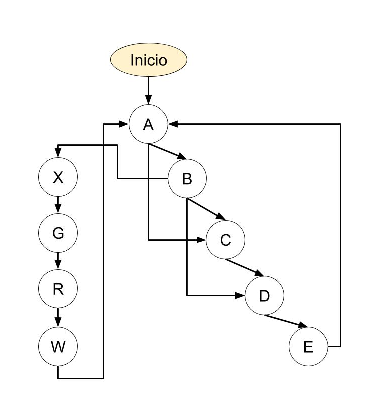
\includegraphics[width=0.5\columnwidth]{chap4/Imagenes/algoritmo2.eps}
\caption{Ejemplo del algoritmo con un grafo dirigido}
\label{fig:alg02}
\end{figure} 
 
Con la anterior definici\'on para los nodos se crea el grafo dirigido,
 siguiendo el algoritmo descrito gr\'aficamente por el diagrama de flujo 
 de la figura \ref{fig:conc01}; cuando se lee una acci\'on se crea el nodo,
 en caso de no existir) y el enlace a est\'e desde el nodo anterior (el nodo
 ra\'iz, para la primer acci\'on le\'ida), y se sigue as\'i durante la sesi\'on
 del usuario. Cuando una acci\'on se repite (es decir, que ya existe el nodo)
 se busca el nodo ya creado correspondiente a dicha acci\'on, se crea el enlace 
 a est\'e nodo y el contador de incidencias de incrementa por la unidad.

\begin{figure}[]
\centering
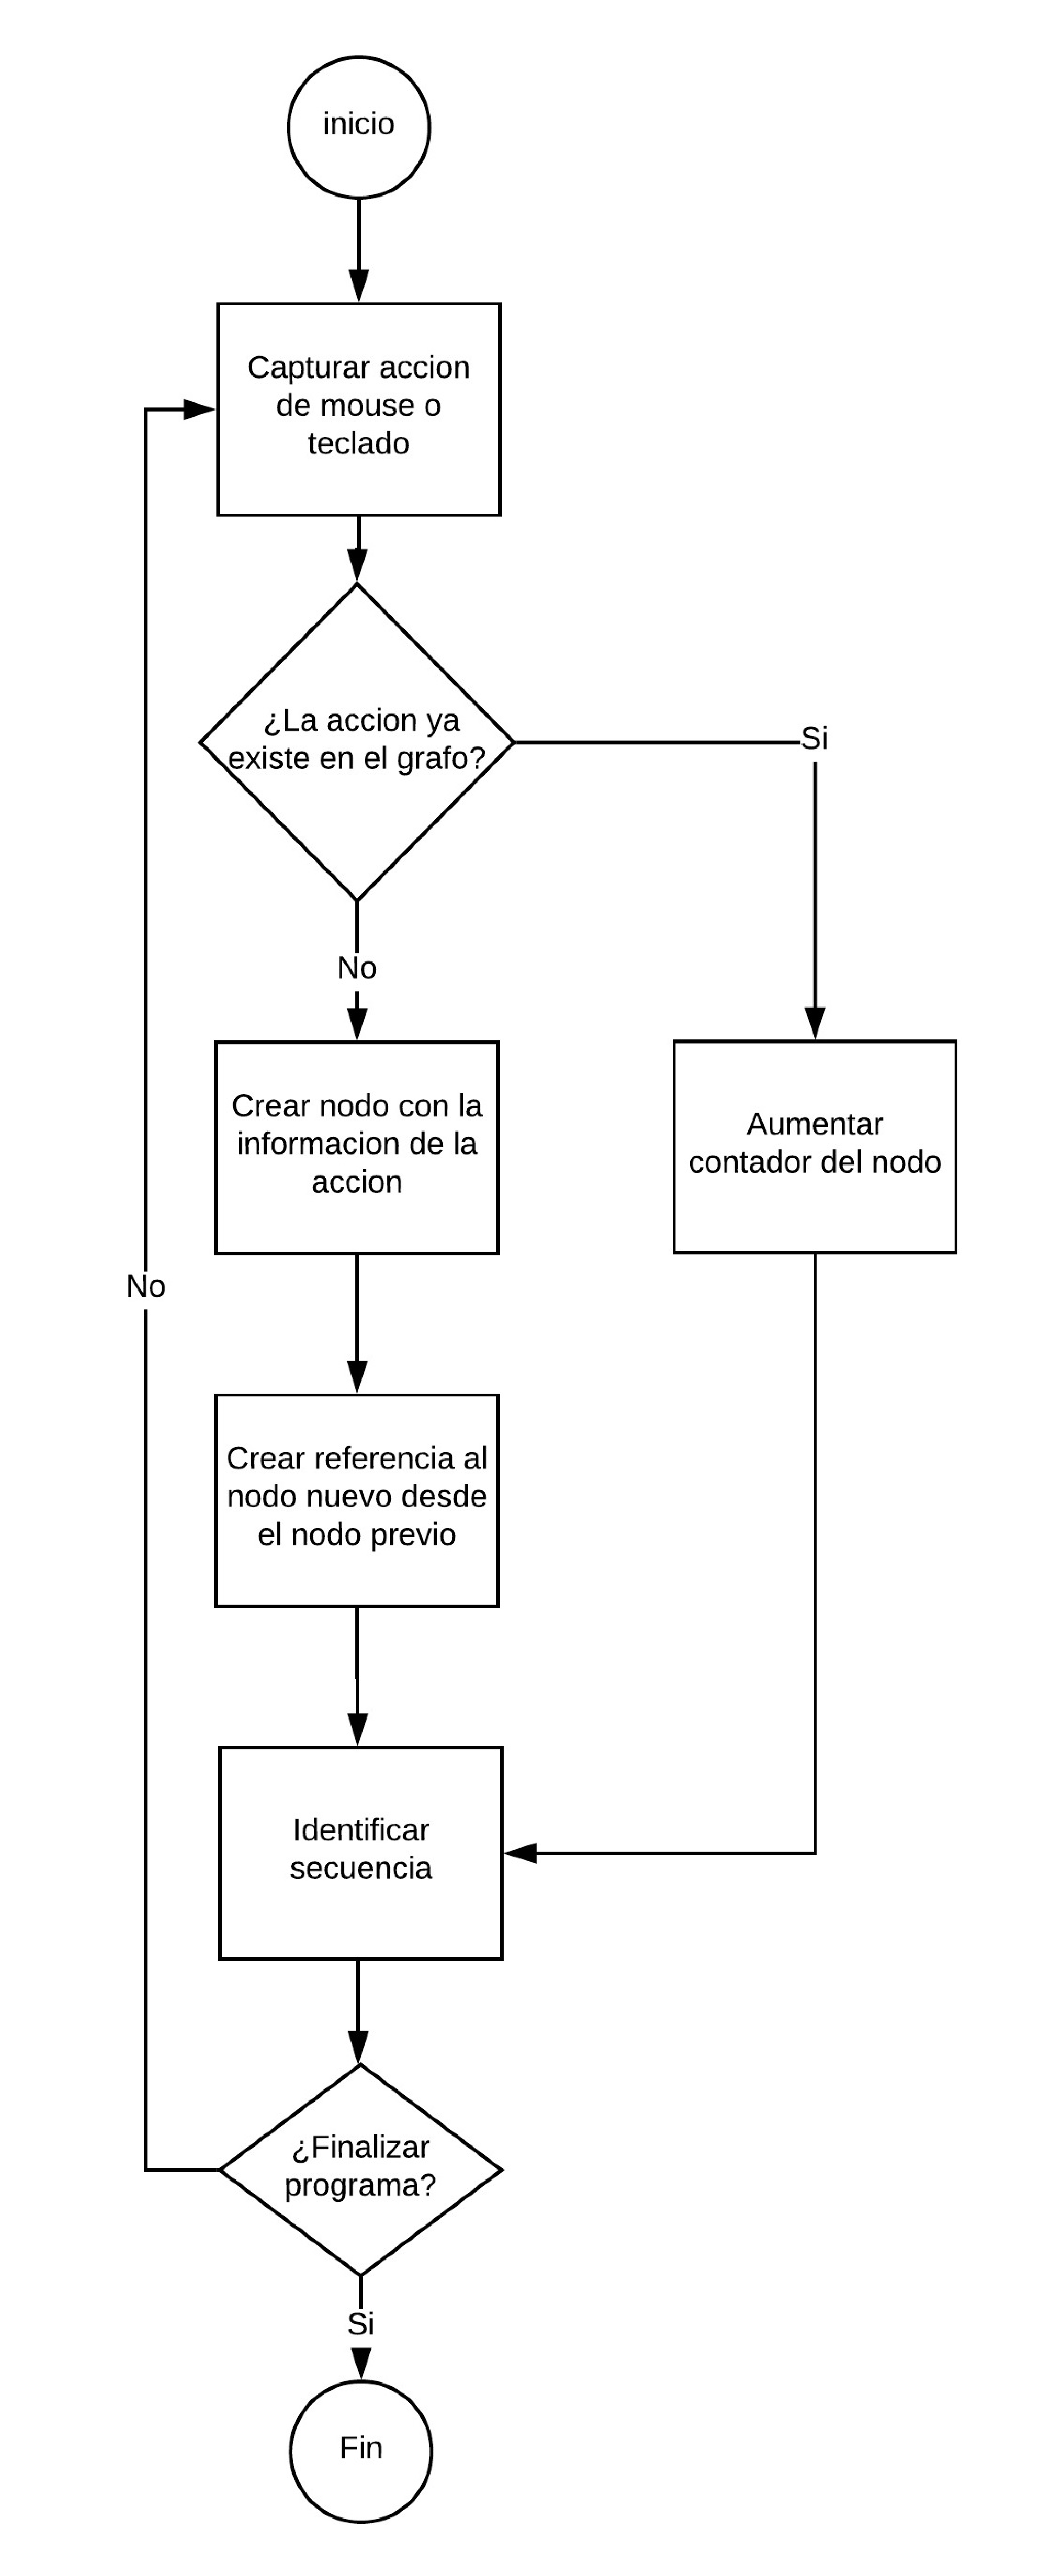
\includegraphics[width=0.5\columnwidth]{chap4/Imagenes/concepto1.eps}
\caption{Diagrama de flujo del algoritmo general}
\label{fig:conc01}
\end{figure} 

El contador de los nodos es utilizado para conocer la frecuencia de cada 
 acci\'on y definir cu\'ales son relevantes, adem\'as, como se puede ver 
 en la figura \ref{fig:conc02}, para obtener una secuencia de acciones se
 genera una lista con las acciones que se est\'an realizando con un numero 
 determinado de incidencias y de forma similar a la analog\'ia con la m\'aquina
 de Turing, al momento de encontrar una acci\'on que se repite en la secuencia,
 se muestra como sugerencia de secuencia \'util y se reinicia la lista, en 
 caso de ser de utilidad a la persona, se guardar\'a para su posterior 
 uso con un nombre significativo para la persona, de lo contrario, la 
 secuencia se guarda para evitar mostrarse nuevamente.

\begin{figure}[]
\centering
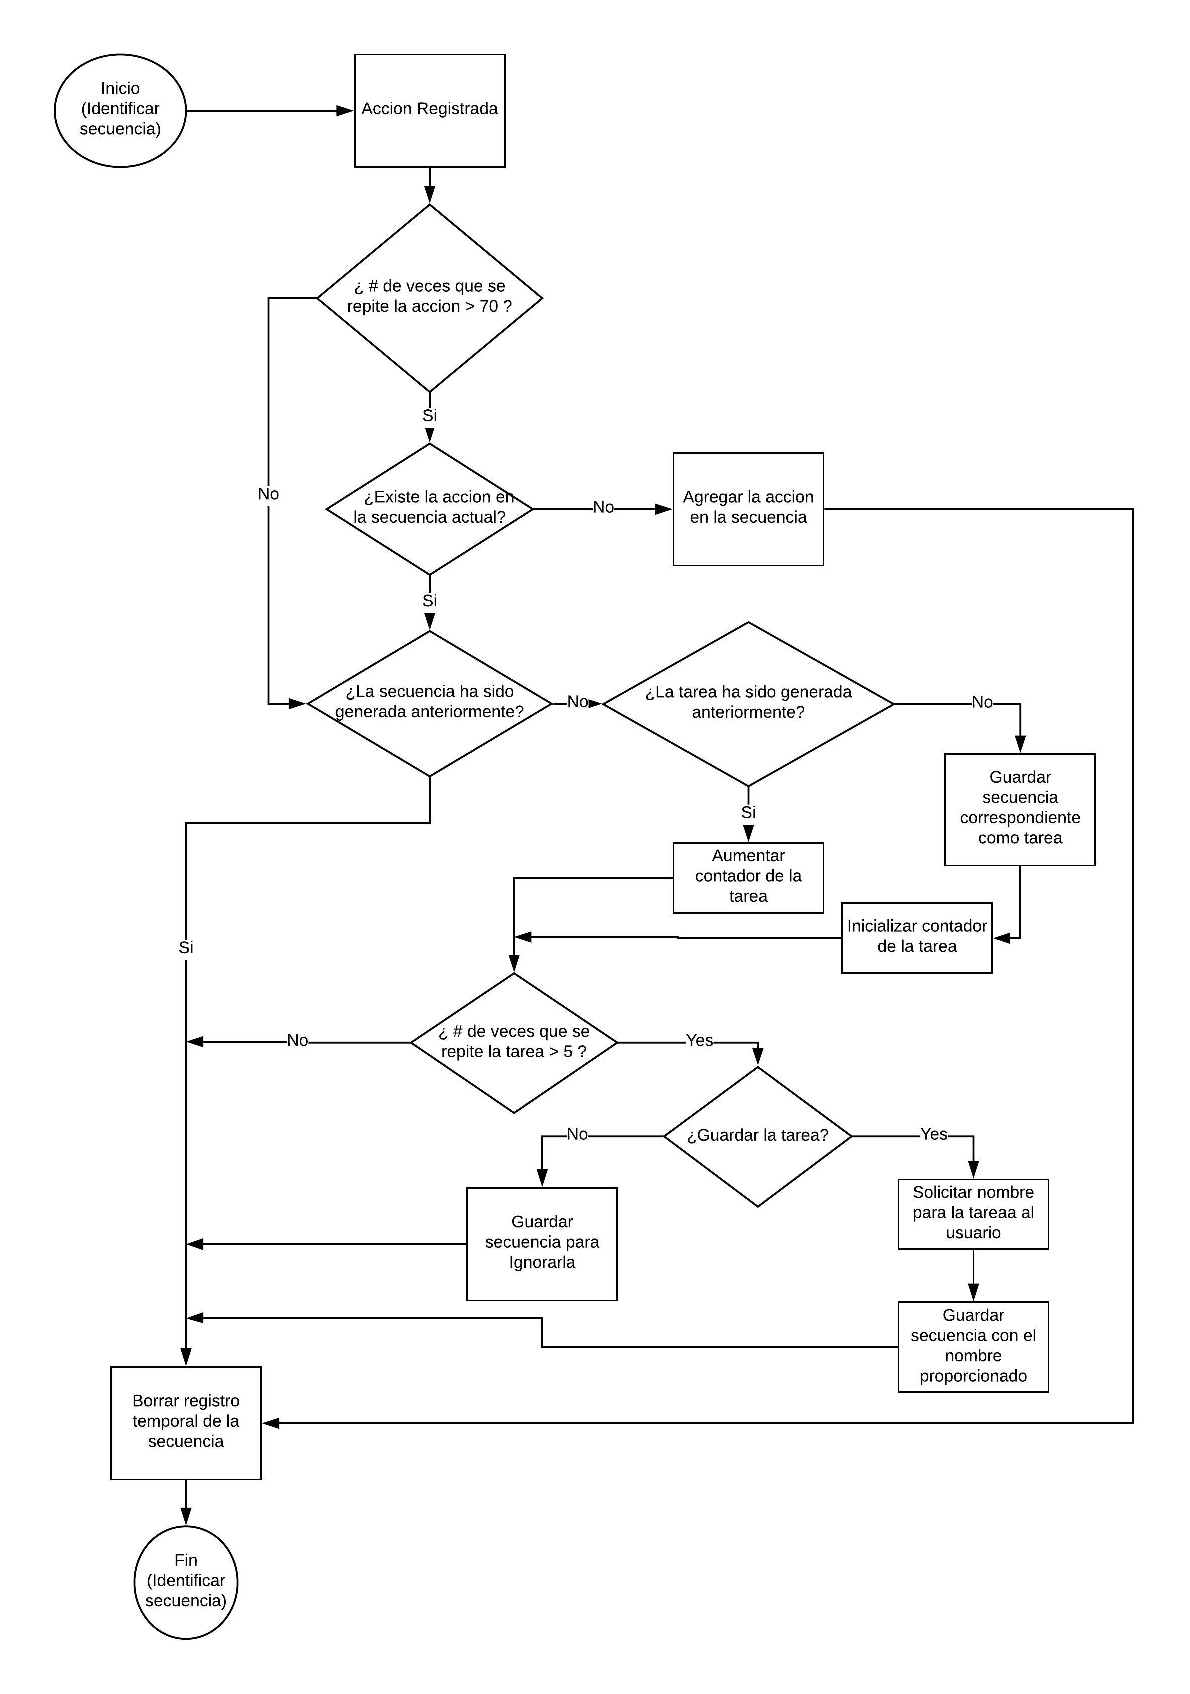
\includegraphics[width=1.0\columnwidth]{chap4/Imagenes/concepto2.eps}
\caption{Diagrama de flujo del bloque ``identificar secuencia'' (ver figura \ref{fig:conc01})}
\label{fig:conc02}
\end{figure} 